\chapter{Visión General del proyecto}

El propósito de este proyecto es desplegar toda la infraestructura de la empresa AlterAid en un dispositivo móvil en nuestro caso una Raspberry Pi. Con la finalidad de poder conseguir desplegar nuestras aplicaciones en lugares remotos o sin conexión a internet o que han sufrido un desastre natural.

Como segundo objetivo del proyecto queremos implementar un pequeño despliegue sensores haciendo que nuestra Raspberry sea el nodo central o sumidero de datos. 
Para poder llevar a cabo todo esto es necesario contar con la utilización de los contenedores usando la tecnología Docker. Que nos facilitaran el trabajo y es motivo de investigación su utilización fuera del mundo de servidores.

\section{Docker}

La idea detrás de Docker es crear contenedores ligeros y portables para las aplicaciones software que puedan ejecutarse en cualquier máquina con Docker instalado, independientemente del sistema operativo que la máquina tenga por debajo, facilitando así también los despliegues.

\begin{figure}[htb]
\begin{center}
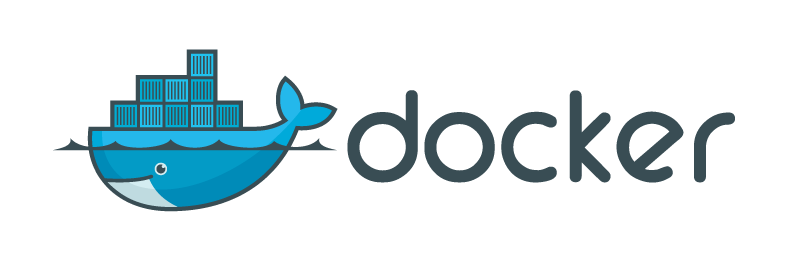
\includegraphics[width=0.5\textwidth]{./setup/dockerLogo}
\caption{Logotipo de Docker}
\label{F:prova}
\end{center}
\end{figure}


\section{Aaaida}
Es una plataforma desarrollada por la empresa AlterAid la cual nos permite crearnos un usuario y con este usuario poder tener varios vínculos. Un Vínculo es un ente que representa aquello por el que el Usuario se ocupa y preocupa. Ejemplos de Vínculos de Usuario pueden ser familiares, pacientes, amigos, etc. 
Esta es una plataforma web la cual recoge todos los datos de las aplicaciones de la empresa y los almacena. Por eso la importancia de poder desplegar toda la infraestructura en un dispositivo que sea fácil de transportar y poder llegar a cualquier lugar.
\newpage
\begin{figure}[htb]
\begin{center}

\includegraphics[width=0.5\textwidth]{./setup/aaaidaLogo}
\caption{Logotipo de Aaaida}
\label{F:prova}
\end{center}
\end{figure}





\section{Motivación}

Conseguir el despliegue de toda la infraestructura de una empresa en un dispositivo de reducidas prestaciones y tamaño como seria una Raspberry Pi, puede abrir campos de investigación y mercado ya que se podrían desarrollar otro tipo de aplicaciones para casos de emergencia o lugares con pocos medios. 
Utilizando una tecnología de servidores como es Docker conlleva un gran avance en el mundo de las IoT.  Un mundo en que las limitaciones tanto de hardware como de software son muy estrictas, nuestro proyecto no es un ejemplo válido ya que el dispositivo utilizado no sería un nodo común utilizado pero sí podría ser un pequeña prueba de concepto para versiones futuras en las cuales se podría utilizar estas tecnologías para facilitar el despliegue de las aplicaciones como de sus actualizaciones ya que al utilizar docker solo se deberia actualizar el contenedor independiente y no todo el sistema.

\section{Objetivos}

Los objetivos fijados para el desarrollo de este proyecto son los siguientes:

\begin{itemize}
\item Analizar y escoger las tecnologías a utilizar para el desarrollo del proyecto
\item La instalaciones de Docker en una Raspberry Pi
\item El despliegue de la infraestructura de la empresa AlterAid
\item La creación de pequeños nodos
\item El despliegue de la red
\item Contemplar la viabilidad de creación de redes smart con estas tecnologías. 
\end{itemize}

\section{Organización del proyecto}

En primer lugar para poder cumplir todos los puntos de los objetivos necesitaremos estudiar un poco más a fondo todas las tecnologías que se pueden utilizar y utilizaremos durante todo el proyecto que serán explicadas en sus capítulos. 

Como se ha explicado previamente se utilizara una Raspberry para desplegar la aplicaciones y esto se hará mediante Docker para ello se tiene que estudiar las diferentes posibilidades, como si es posible ejecutar docker en un sistema ARM, si se podrá virtualizar la Raspberry para poder hacer las pruebas de una manera mas comoda etc. todo se podrá ver en sus capítulos, capítulo 2 y capítulo 3. 

Una vez solucionado todos los problemas de desplegar la aplicación y ejecutarla, para poder arrancar aaaida, en el capítulo 4 podremos ver una pequeña explicación del funcionamiento de la plataforma y sus funcionalidades. 

Para terminar la parte técnica, vendría el paso de crear la red de sensores para poder comunicarnos con la Raspberry una vez se haya llevado a cabo esta conexión el envío de los datos y su correcto almacenamiento para poder ser visualizados en la plataforma aaaida todo esto se comentará en el capítulo 5. 

Por último, con la plataforma en la Raspberry y la red de sensores funcionando obtendremos el último capítulo donde se podrán ver las conclusiones y resultados sobre la viabilidad de este proyecto. 

